%%%% ijcai15.tex

\typeout{IJCAI-15 Instructions for Authors}

% These are the instructions for authors for IJCAI-15.
% They are the same as the ones for IJCAI-11 with superficical wording
%   changes only.

\documentclass{article}
% The file ijcai15.sty is the style file for IJCAI-15 (same as ijcai07.sty).
\usepackage{ijcai15, graphicx, times}

% the following package is optional:
%\usepackage{latexsym} 

% Following comment is from ijcai97-submit.tex:
% The preparation of these files was supported by Schlumberger Palo Alto
% Research, AT\&T Bell Laboratories, and Morgan Kaufmann Publishers.
% Shirley Jowell, of Morgan Kaufmann Publishers, and Peter F.
% Patel-Schneider, of AT\&T Bell Laboratories collaborated on their
% preparation.

% These instructions can be modified and used in other conferences as long
% as credit to the authors and supporting agencies is retained, this notice
% is not changed, and further modification or reuse is not restricted.
% Neither Shirley Jowell nor Peter F. Patel-Schneider can be listed as
% contacts for providing assistance without their prior permission.

% To use for other conferences, change references to files and the
% conference appropriate and use other authors, contacts, publishers, and
% organizations.
% Also change the deadline and address for returning papers and the length and
% page charge instructions.
% Put where the files are available in the appropriate places.

\title{GraphEvol: A Graph Evolution Technique for Web Service Composition}

\author{Alexandre Sawczuk da Silva, Hui Ma, Mengjie Zhang\\ School of
Engineering and Computer Science, Victoria University of Wellington, New Zealand\\
\{Alexandre.Sawczuk.da.Silva, Hui.Ma, Mengjie.Zhang\}@ecs.vuw.ac.nz}

%\author{Qiang Yang \\
%Hong Kong University of Science and Technology\\
%Hong Kong, China \\
%pcchair15@ijcai.org}

\begin{document}

\maketitle

\begin{abstract}
  The {\it IJCAI--15 Proceedings} will be printed from electronic
  manuscripts submitted by the authors. The electronic manuscript will
  also be included in the online version of the proceedings. This paper
  provides the style instructions.
\end{abstract}

\section{Introduction}

A Web service can be defined as a software module that accomplishes a specific task and that is made available for requests over
the Internet. The fundamental benefit of such modules is that they can be interwoven with new applications, preventing developers from rewriting
functionality that has already been implemented. Service-Oriented Architecture (SOA) is a paradigm that expands on this idea, advocating
that the main atomic components of a software system should be Web services, since this maximizes code reuse and information sharing.
As services are typically present standard interfaces, the possibility arises to create approaches capable of combining services
automatically according to the final desired system, in a process known as \textit{Web service composition}. The objective of these approaches
is to produce a workflow, i.e. a directed acyclic graph (DAG), stipulating the sequence in which each atomic service should be executed, as well as
the output-input connections between services.

Many approaches to Web service composition have been proposed in the literature, from variations on AI planning techniques to the employment
of integer linear programming solvers. In particular, promising results have been achieved with the use of Evolutionary Computation (EC) techniques,
because their search methods successfully handle the large search space characteristic of the composition problem. Existing evolutionary
techniques for fully automated Web service composition can be divided into two different groups according to the extent of the composition they
perform: \textit{semi-automated composition techniques}, assume that a general workflow of abstract tasks has already been provided and that the
algorithm must simply find the best candidate for each task slot; \textit{fully automated composition techniques}, on the other hand, make no such
assumption, meaning that they construct the task workflow and select the most suitable candidates simultaneously. Because of their greater capabilities,
fully automated composition techniques are the focus of this paper.

While semi-automated composition can be accomplished using a variety of techniques such as Genetic Algorithms (GA) and Particle Swarm Optimisation
(PSO) \cite{}, fully automated composition using EC is currently mostly restricted to techniques employing the traditional Genetic Programming (GP) model \cite{rodriguez2010composition}.
In this paradigm, each each composition candidate is a tree that represents an underlying graph solution that can be obtained through a translation
process. The question then arises whether it is possible to represent a candidate directly as a graph, and whether the system's performance is affected
from doing so. Thus, the objective of this paper is to present and analyse \textit{GraphEvol}, an evolutionary computation technique for Web service
composition where each candidate is represented as a DAG and modified while remaining in that form. The remainder of this paper is organised as follows:
Section \ref{background} presents background information concerning Web service composition; Section \ref{graphevol} presents the proposed technique;
Section \ref{experimentdesign} discusses the experiments conducted to compare the performance GraphEvol to that of a GP composition approach;
Section \ref{results} describes the experiment results; Section \ref{conclusions} concludes the paper.

\section{Background}\label{background}

\subsection{The Web Service Composition Problem}
In a standard composition problem, a user would like to obtain a composite Web service with a particular functionality. The user makes a request to a Web
service composition system specifying the \textit{inputs} the composite service should accept, the \textit{outputs} it should produce, the \textit{constraints}
it should consider (e.g. the resulting composite service should have the lowest possible execution time), and the \textit{repository} from which it should select
the atomic services to include in the composition. Given this information, the composition system \textit{discovers} relevant services from the repository, and uses
these services as potential candidates to be included in the final composition. A composition algorithm is run to \textit{select} appropriate services at the same
time it \textit{builds} a workflow denoting how each service in the composition interacts with the others with regards to their required input and produced output.

A classic example of automated Web service composition is the travel planning scenario \cite{srivastava2003web}, where the objective is to create a system capable of
automatically reserving hotels and flights according to customer preferences. In this scenario the customer preference types, such as departure date and destination
city, are the composition \textit{inputs}, and the reservation outcomes, such as issued tickets and receipts, are the composition \textit{outputs}. The relevant composition
candidates are a set of hotel and flight booking services that are to be combined into a cohesive task workflow by the composition system. Figure \ref{fig:compositionExample} shows a simple composition solution that performs flight and hotel reservations according to a customer's information. More specifically, when using this composite service 
the customer provides her/his personal information and travel details, such as the departure date, the destination city and the duration of the stay. This information is
then used to book return flight tickets, and to determine the customer's arrival date at the destination city.

\begin{figure}
\centerline{
\fbox{
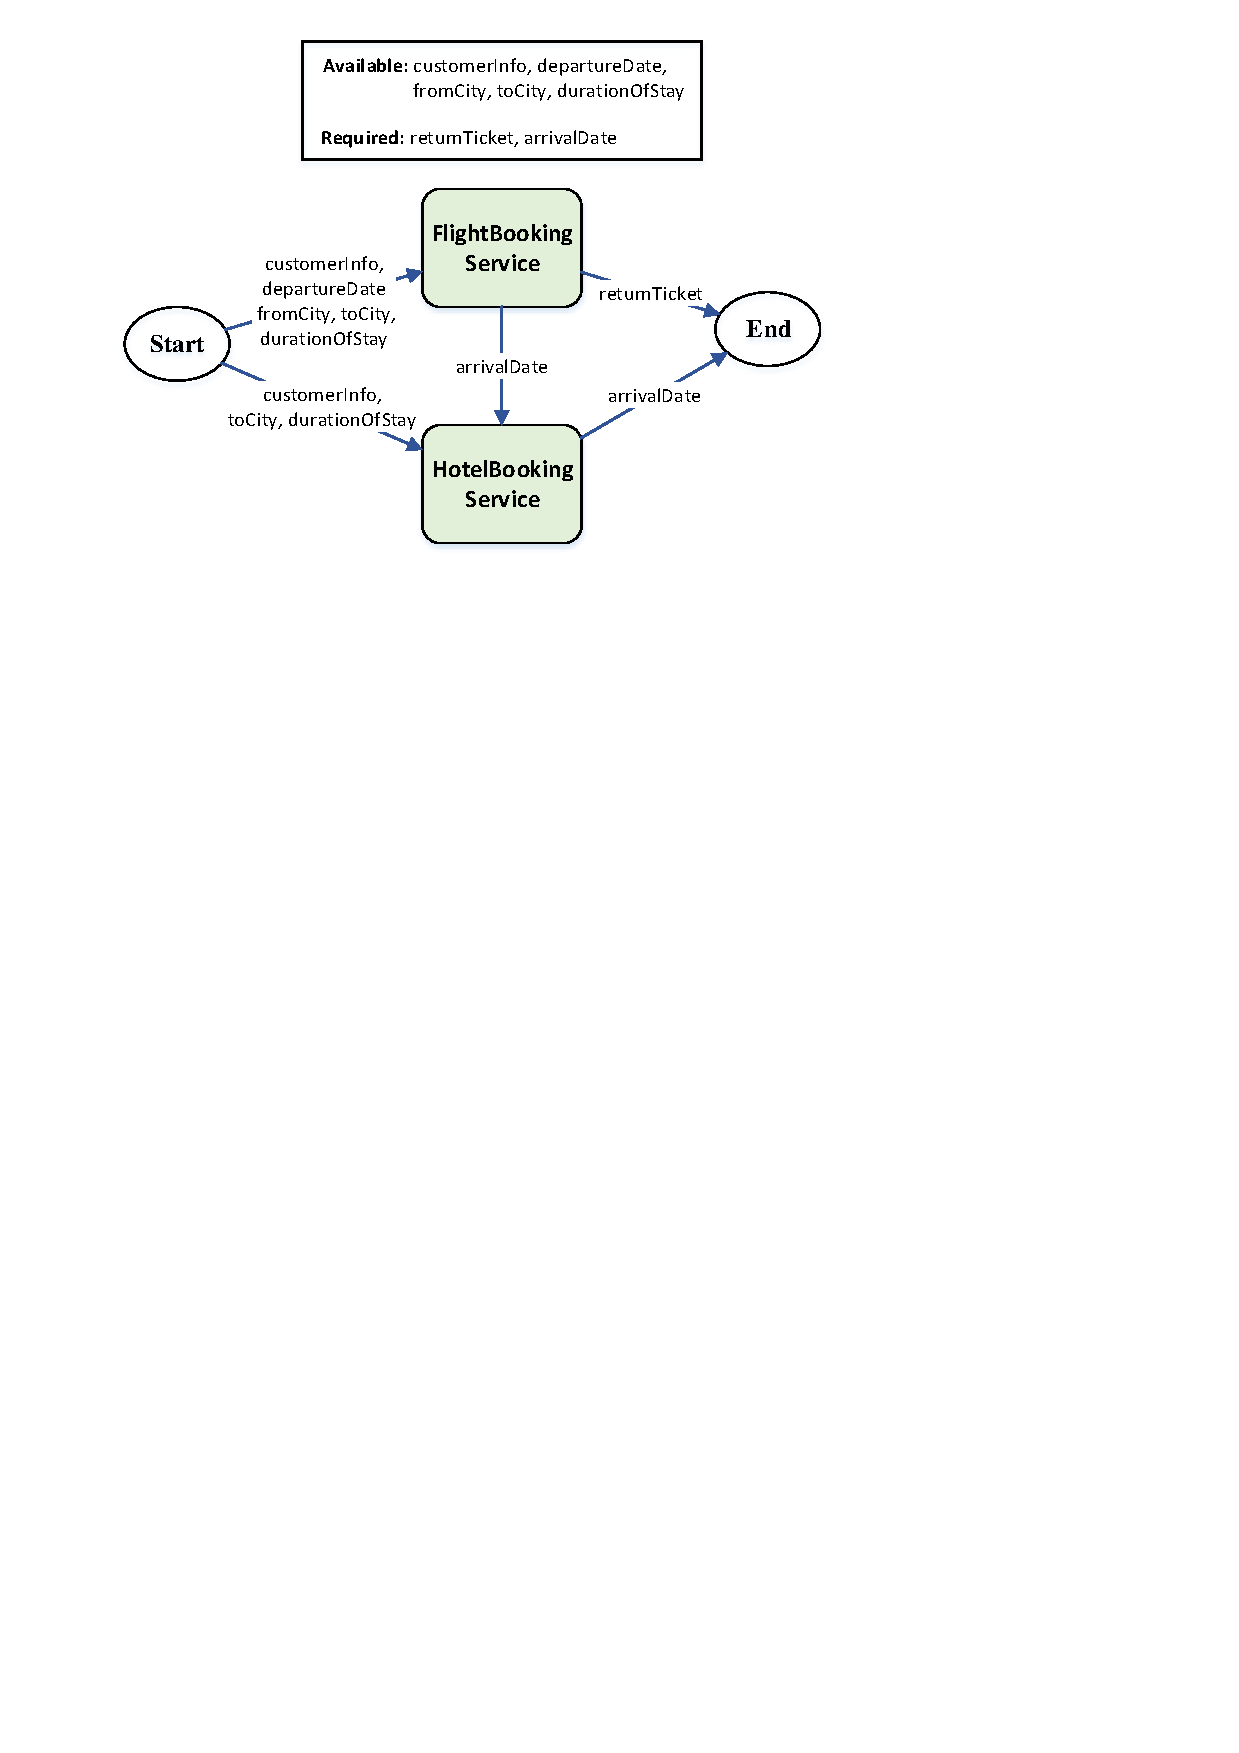
\includegraphics[width=8cm]{compositionExample.pdf}}}
\caption{Example of a solution to a Web service composition task.}
\label{fig:compositionExample}
\end{figure}

\subsection{Related Work}
There are many publications on the subject of EC applied to Web service composition, but this Subsection will focus on those which perform fully automated composition,
since their composition outcomes are analogous to those of GraphEvol. One of the pioneering GP composition approaches \cite{aversano2006genetic} uses workflow constructs as the non-terminal tree nodes and Web service candidates as the terminal nodes, where workflow constructs represent the output-input connections between
two services. For example, if two services are sequentially connected, so that output of service \textit{A} is used as the input of service \textit{B}, this would be represented
by a \textit{sequence} workflow construct having \textit{A} as the left child and \textit{B} as the right one. Likewise, if two services \textit{A} and \textit{B} have independent inputs and outputs and can be executed in parallel, this can be encoded as a \textit{flow} construct having \textit{A} and \textit{B} as its children. An example of a tree generated by this technique is shown in Figure \ref{fig:treeExample}, adapted from an illustration in the referenced work. The initial population is initialised randomly, which means that the initial compositions represented in that generation are very unlikely to be executable, since their inputs and outputs are mismatched. The aim of the technique is to improve these output-input matches by employing a fitness function that calculates their correspondence and awards higher fitness scores to those candidates with larger overlaps. The genetic operators employed for this evolutionary process are crossover, where two subtrees from two individuals are randomly selected and swapped, and mutation, where a subtree for an individual is replaced with a randomly generated substitute.

Another GP approach \cite{rodriguez2010composition} follows a similar tree representation to the one discussed above, as well as a similar implementation of mutation and crossover operators. The greatest distinction between this approach and others is in its use of a context-free grammar to generate the initial population of candidates and to create the subtrees used during mutation. The grammar restricts the tree structure configurations allowed in the tree, thus reducing the search space considered when searching for a solution. Another key difference of this approach is in its fitness function, which not only minimises the output-input mismatches in candidates, but also minimises the overall number of atomic services in the composition and the size of the largest sequential chain of such services. These two additions to the fitness function are aimed at reducing the overall execution time and cost of the resulting compositions. This technique was tested against two well-known semantically-annotated datasets, OWL-S TC \cite{kuster2008opossum} and WSC2008 \cite{bansal2008wsc}, showing that it yields valid solutions to all composition tasks while requiring a relatively low amount of execution time.

\begin{figure}
\centerline{
\fbox{
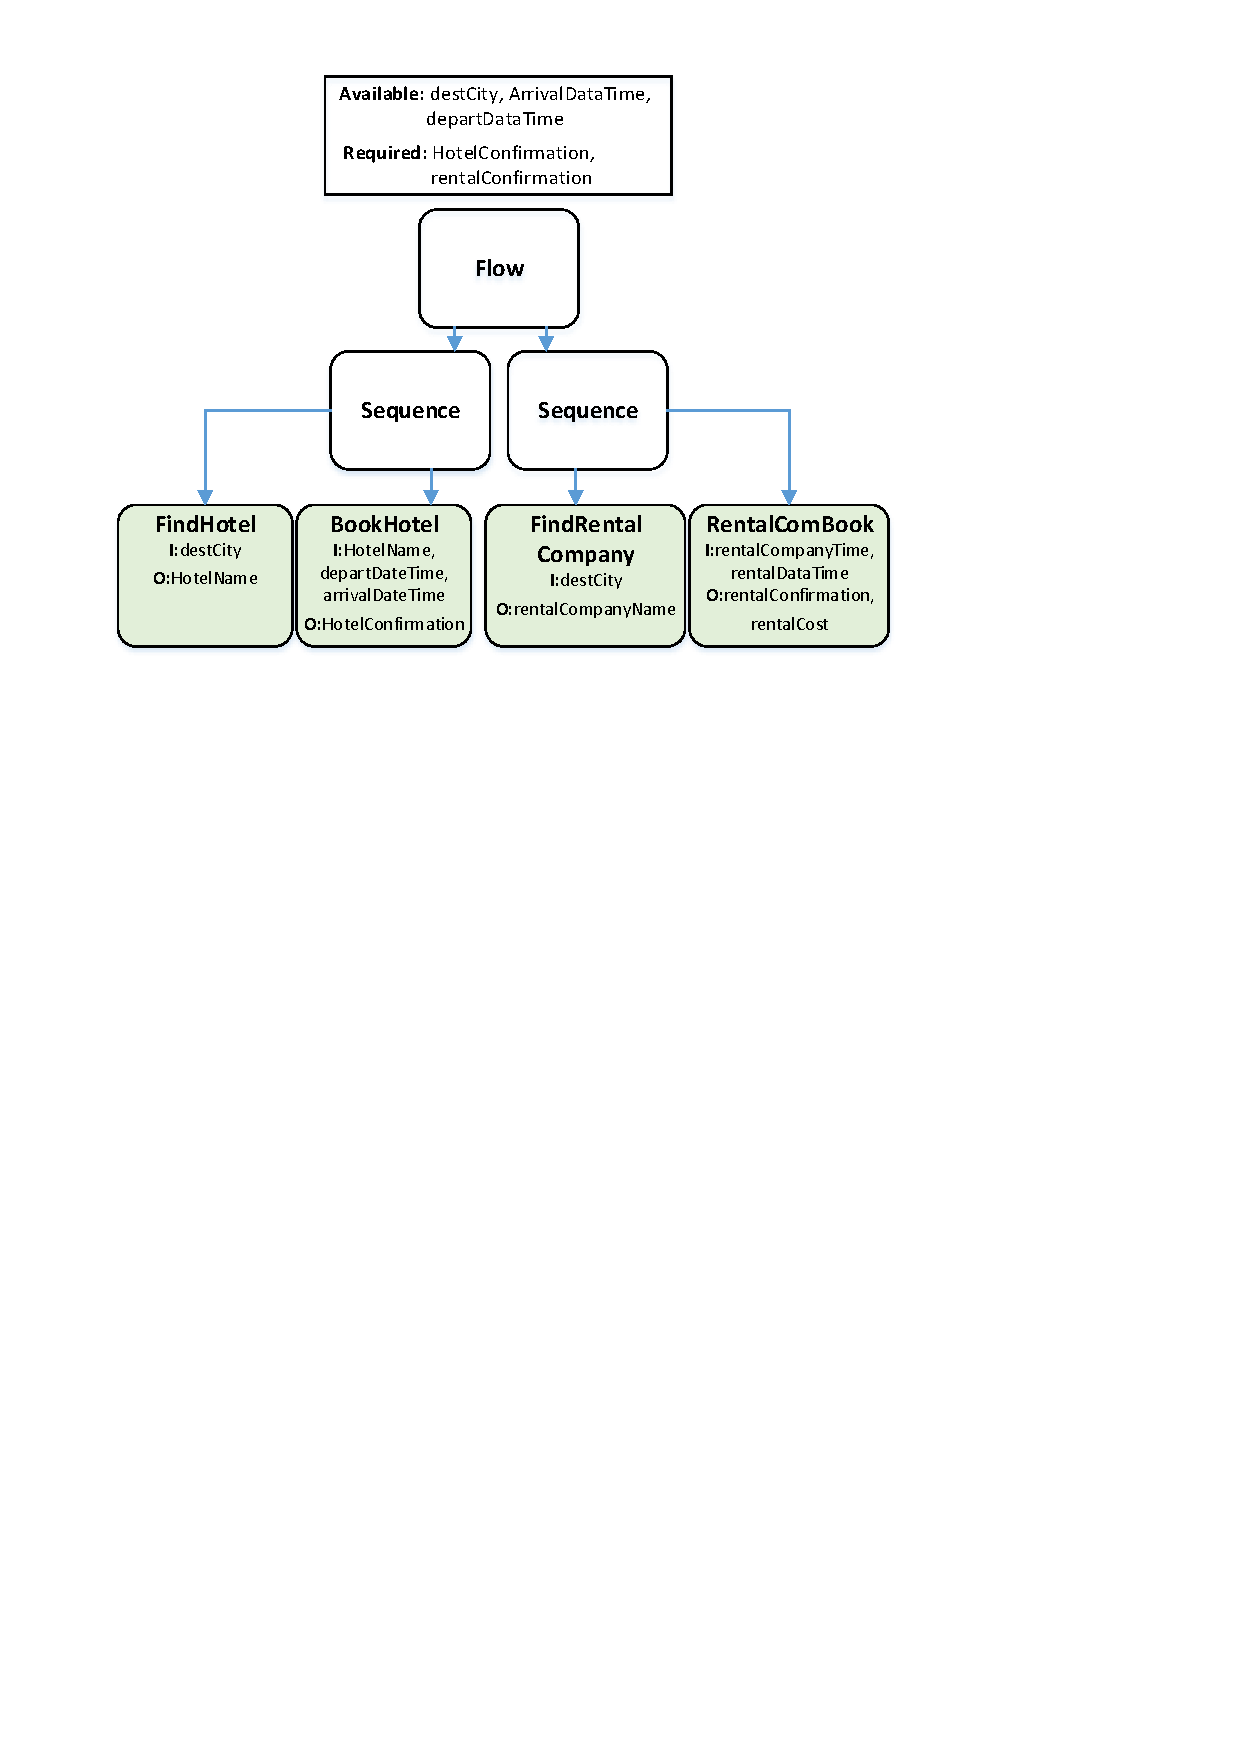
\includegraphics[width=8cm]{treeExample.pdf}}}
\caption{Example of a typical GP candidate composition tree \protect\cite{aversano2006genetic}.}
\label{fig:treeExample}
\end{figure}

In addition to GP, an approach using PSO has also been shown to be a suitable method for fully automated Web service composition \cite{silva2014graph}. In this technique, candidates encoded as a vectors of weights (particles), each ranging from 0 to 1. These weights are mapped to the edges of a \textit{master graph}, which is a data structure created at 
initialisation time to represent all the possible output-intput relationships between relevant candidate services. The central idea of this technique is to utilise a greedy algorithm
to extract non-redundant functional solutions from the master graph, using the weights as guides that prioritise the choice of certain edges and nodes of the structure. The weights
are evolved using the classical PSO algorithm, and at each generation the fitness of all solutions is calculated by extracting the underlying structure from the master graph. Since
the master graph structure is built ensuring full matching of services inputs and outputs, the fitness function employed for evolution optimises the population according to non-functional quality (QoS) measures such as response time, availability, and reliability.

\section{GraphEvol}\label{graphevol}
GraphEvol, the evolutionary computation approach proposed in this work, bears many similarities with the GP approaches discussed above. Namely, it initialises and a population 
of candidates that are encoded using non-linear data structures, evolves this population using crossover and mutation operators, and evaluates the quality of each candidate
based on the nodes included in its structure. However, as opposed to representing candidate compositions as trees that correspond to underlying graph structures, GraphEvol
represents them directly as graphs. As a consequence, the mutation and crossover operators must be implemented differently, and so must the fitness function.


\section{Experiment Design}\label{experimentdesign}

\section{Results}\label{results}

\section{Conclusions}\label{conclusions}

%% The file named.bst is a bibliography style file for BibTeX 0.99c
\bibliographystyle{named}
\bibliography{ijcai15}

\end{document}

